
%%%%%%%%%%%%%%%%%%%%%%%%%%%%%%%%%%%%%%%%%%%%%%%%%%%%%%%%%%%%%%%%%%%%%%%
%%%%%%%%%%%%%%%%%%%%%%%%%%%%%%%%%%%%%%%%%%%%%%%%%%%%%%%%%%%%%%%%%%%%%%% 
%%%%%%%%%%%       								 Preamble				         	                                                        %%%%%%%%%% 
%%%%%%%%%%%%%%%%%%%%%%%%%%%%%%%%%%%%%%%%%%%%%%%%%%%%%%%%%%%%%%%%%%%%%%% 
%%%%%%%%%%%%%%%%%%%%%%%%%%%%%%%%%%%%%%%%%%%%%%%%%%%%%%%%%%%%%%%%%%%%%%% 
\documentclass[10pt]{beamer}
\usepackage{setspace}
\usepackage{color}
\usepackage{amsmath,lmodern}
\usepackage{hyperref}
\usepackage{graphicx}
\usepackage{multirow}
\usepackage{tikz}
\usetikzlibrary{fit,shapes.misc}
\usepackage{pdflscape}
\usepackage{amsmath}
\usepackage{lscape}
\usepackage{multirow}
\usepackage{enumerate}
\usepackage{epstopdf}
\usepackage{pdfpages}
\usepackage{appendixnumberbeamer}
\usepackage{color,soul}
\usepackage{grffile}
\usepackage{float}
\usepackage{relsize}
\usepackage{tcolorbox}
\newcounter{nodemarkers}
\usepackage{tikz}
\newcommand{\toplinesmall}{%
  \tikz[remember picture,overlay] {%
    \draw[blue,thick] ([yshift=-1cm, xshift=.9cm]current page.north west)
             -- ([yshift=-1cm,xshift=3.6cm]current page.north west);}}
             
\newcommand{\toplinemedium}{%
  \tikz[remember picture,overlay] {%
    \draw[blue,thick] ([yshift=-1cm, xshift=.9cm]current page.north west)
             -- ([yshift=-1cm,xshift=6.2cm]current page.north west);}}
 
 \newcommand{\toplinelarge}{%
  \tikz[remember picture,overlay] {%
    \draw[blue,thick] ([yshift=-1cm, xshift=.9cm]current page.north west)
             -- ([yshift=-1cm,xshift=8.9cm]current page.north west);}}           
             
 \newcommand{\toplinexlarge}{%
  \tikz[remember picture,overlay] {%
    \draw[blue,thick] ([yshift=-1cm, xshift=.9cm]current page.north west)
             -- ([yshift=-1cm,xshift=12cm]current page.north west);}}                       
             
\setbeamertemplate{footline}
{
  \leavevmode%
  \hbox{%
  \begin{beamercolorbox}[wd=.333333\paperwidth,ht=2.25ex,dp=1ex,center]{author in head/foot}%
    \usebeamerfont{author in head/foot}{\textcolor{blue}{ECON311}}
  \end{beamercolorbox}%
  \begin{beamercolorbox}[wd=.333333\paperwidth,ht=2.25ex,dp=1ex,center]{title in head/foot}%
    \usebeamerfont{title in head/foot}{\textcolor{blue}{Winter 2026}}
  \end{beamercolorbox}%
  \begin{beamercolorbox}[wd=.333333\paperwidth,ht=2.25ex,dp=1ex,right]{date in head/foot}%
    \usebeamerfont{date in head/foot}{\textcolor{blue}{Lecture 6 \: \: \: \: \: \: \: }
    \insertframenumber{} / \inserttotalframenumber\hspace*{2ex}} 
  \end{beamercolorbox}}%
  \vskip0pt%
}
\newtheorem{proposition}[theorem]{Proposition}

\newcommand\marktopleft[1]{%
    \tikz[overlay,remember picture] 
        \node (marker-#1-a) at (-0.2,1.2ex) {};%
}
\newcommand\markbottomright[1]{%
    \tikz[overlay,remember picture] 
        \node (marker-#1-b) at (0.16,-1ex) {};%
    \tikz[overlay,remember picture,thick,inner sep=4pt]
        \node[draw,rectangle,rounded corners, blue, fit=(marker-#1-a.center) (marker-#1-b.center)] {};%
}

\setbeamertemplate{caption}{\raggedright\insertcaption\par}
\setbeamertemplate{itemize items}[ball]
\setbeamertemplate{itemize subitem}[triangle]
\setbeamertemplate{itemize subsubitem}[triangle]
\tcbset{colframe=white,colback=white,nobeforeafter}
\beamertemplatenavigationsymbolsempty
\addtobeamertemplate{frametitle}{\vspace*{0.19cm}}{\vspace*{0cm}}


%%%%%%%%%%%%%%%%%%%%%%%%%%%%%%%%%%%%%%%%%%%%%%%%%%%%%%%%%%%%%%%%%%%%%%%
%%%%%%%%%%%%%%%%%%%%%%%%%%%%%%%%%%%%%%%%%%%%%%%%%%%%%%%%%%%%%%%%%%%%%%% 
%%%%%%%%%  									    Define Title									                                       %%%%%%%%%
%%%%%%%%%%%%%%%%%%%%%%%%%%%%%%%%%%%%%%%%%%%%%%%%%%%%%%%%%%%%%%%%%%%%%%%
%%%%%%%%%%%%%%%%%%%%%%%%%%%%%%%%%%%%%%%%%%%%%%%%%%%%%%%%%%%%%%%%%%%%%%% 
\title{ECON 311} 
\author{Lecture 6: Solow Growth Model}
\date{}
\AtBeginSection[]
{
 \begin{frame}<beamer>
 \tableofcontents[currentsection]
 \end{frame}
}
%%%%%%%%%%%%%%%%%%%%%%%%%%%%%%%%%%%%%%%%%%%%%%%%%%%%%%%%%%%%%%%%%%%%%%%
%%%%%%%%%%%%%%%%%%%%%%%%%%%%%%%%%%%%%%%%%%%%%%%%%%%%%%%%%%%%%%%%%%%%%%% 
%%%%%%%% 						     				Document								                                                %%%%%%%%
%%%%%%%%%%%%%%%%%%%%%%%%%%%%%%%%%%%%%%%%%%%%%%%%%%%%%%%%%%%%%%%%%%%%%%%
%%%%%%%%%%%%%%%%%%%%%%%%%%%%%%%%%%%%%%%%%%%%%%%%%%%%%%%%%%%%%%%%%%%%%%% 
\begin{document}
\setbeamercovered{transparent}

\begin{frame}
\maketitle
\end{frame}

%%%%%%%%%%%%%%%%%%%%%%%%%%%%%%%%%%%%%%%%%%%%%%%%%%%%%%%%%%%%%%%%%%%%%%%
%%%%%%%%%%%%%%%%%%%%%%%%%%%%%%%%%%%%%%%%%%%%%%%%%%%%%%%%%%%%%%%%%%%%%%% 
%%%%%%%% 						     				Introduction	             		                                		  %%%%%%%%
%%%%%%%%%%%%%%%%%%%%%%%%%%%%%%%%%%%%%%%%%%%%%%%%%%%%%%%%%%%%%%%%%%%%%%%
%%%%%%%%%%%%%%%%%%%%%%%%%%%%%%%%%%%%%%%%%%%%%%%%%%%%%%%%%%%%%%%%%%%%%%% 


\section{The Solow Growth Model}

\begin{frame}
\frametitle{\: \: \: Introduction} \label{solow}
\toplinemedium
\begin{itemize}
\item The production model is very useful because is able to display two features of the data:
\begin{enumerate}
\vspace{.11in} 
\item $\frac{y_{ind}}{y_{nind}}=\frac{\overline{A}_{ind} \left(\overline{k}_{ind}\right)^{\frac{1}{3}}}{\overline{A}_{nind} \left(\overline{k}_{nind}\right)^{\frac{1}{3}}}$ (differences in levels of $y$)  
\vspace{.2in} 
\item $g_{y_{ind}}-g_{y_{nind}}=(g_{\overline{A}_{ind}}+\frac{1}{3} g_{\overline{k}_{ind}})-(g_{\overline{A}_{nind}}+\frac{1}{3}g_{\overline{k}_{nind}})$ (differences in growth rates of $y$)  \hyperlink{growth}{\beamerbutton{Growth Algebra}}
\end{enumerate}
\vspace{.11in} 
\item Nevertheless, it does not provide any explanation as to why the growth rates are so different across countries.
\begin{itemize}
\vspace{.11in} 
\item The Solow Model provides an explanation for $K$ accumulation, which will help us to explain why capital per worker grows at a faster pace in some countries.
\vspace{.11in} 
\item As we have seen this is only a part of the explanation, but it is a very useful starting point for understanding the big differences in growth rates we observe in the data.   
\end{itemize}
\end{itemize}
\end{frame}

\begin{frame}
\frametitle{\: \: \: Capital Accumulation}
\toplinemedium
\begin{itemize}
\item At the center of the Solow Model is the capital accumulation equation:
\begin{eqnarray*}
K_{t+1}=I_t+(1-\overline{d})K_t
\end{eqnarray*}
\begin{itemize}
\item $I$=investment, $\overline{d}$=depreciation rate ($0 \leq \overline{d} \leq 1$)
\end{itemize}
\vspace{.11in}
\item We can rewrite this equation in changes: $\Delta K_{t+1}=K_{t+1}-K_t$:
\begin{columns}
\begin{column}{0.4\linewidth}
\begin{eqnarray*}
\Delta K_{t+1}=I_t-\overline{d}K_t:
\end{eqnarray*}
\end{column}
\begin{column}{0.7\linewidth}
\begin{figure}
\centering
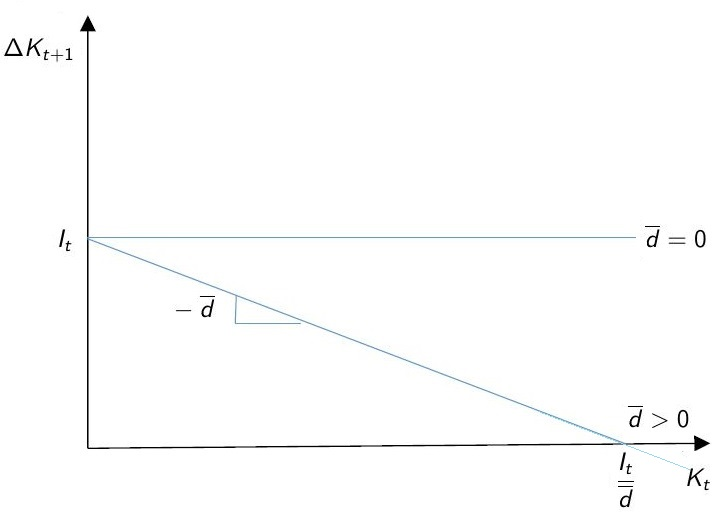
\includegraphics[scale=.28]{lom}
\end{figure}
\end{column}
\end{columns}
\end{itemize}
\end{frame}

\begin{frame}
\frametitle{\: \: \: Capital Accumulation}
\toplinemedium
\begin{itemize}
\item Investing in capital for $t+1$ requires resources at $t$:
\begin{eqnarray*}
C_t+I_t=Y_t \: \: \: \: \: (\text{resource constraint})
\end{eqnarray*}
\begin{itemize}
\item An assumption of the Solow model is that capital and consumption goods are produced using the same production function.
\vspace{.11in}
\end{itemize}
\item We are going to assume that individual decisions to save and invest is exogenous:
\begin{eqnarray*}
\begin{array}{lcl}
I_t=\overline{s} Y_t \: \: \: \: \: (\text{allocation of resources}) &,&0 \leq \overline{s} \leq 1
\end{array} 
\end{eqnarray*}
\item Combining the allocation of resources with the capital accumulation equation, we obtain:
\only<1>{\begin{eqnarray*}
\Delta K_{t+1}=\overline{s} Y_t-\overline{d}K_t \: \: \: \: \: (\text{law of motion})
\end{eqnarray*}}
\only<2>{\begin{eqnarray*}
\Delta K_{t+1}=\overline{s} F(K_t,L_t)-\overline{d}K_t \: \: \: \: \: (\text{law of motion})
\end{eqnarray*}}
\end{itemize}
\end{frame}

\begin{frame}
\frametitle{\: \: \: Dynamics of Capital Accumulation}
\toplinexlarge
\only<1>{\begin{figure}
\centering
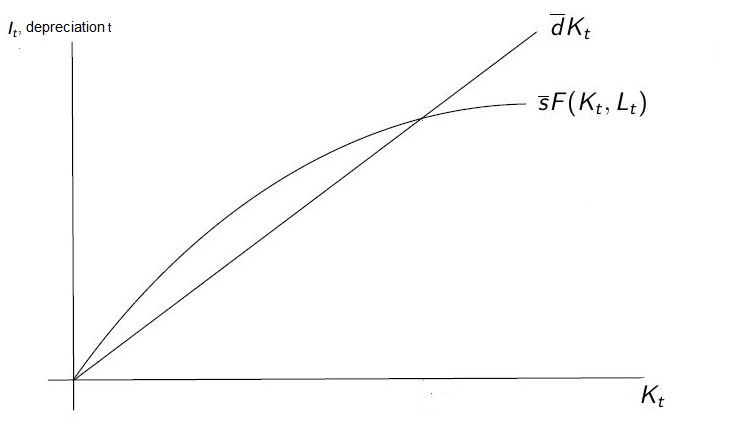
\includegraphics[scale=.6]{basic_solow}
\caption{$\Delta K_{t+1}=\overline{s} F(K_t,L_t)-\overline{d}K_t $}
\end{figure}}
\only<2>{\begin{figure}
\centering
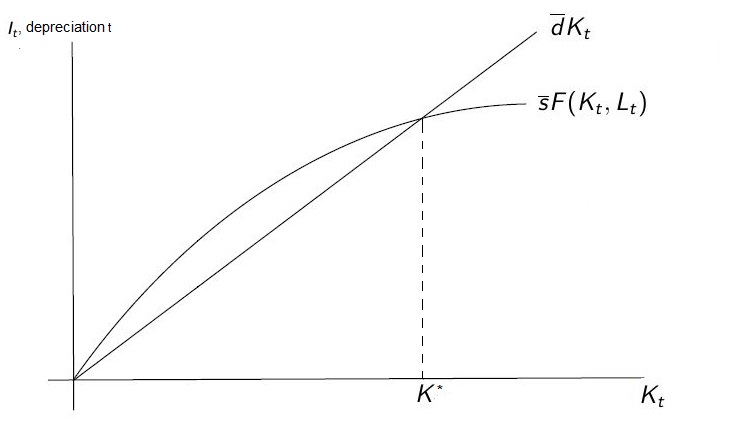
\includegraphics[scale=.6]{basic_solow_2}
\caption{$\underbrace{\Delta K_{t+1}}_{K_{t+1}=K_t}=0  \Leftrightarrow  \underbrace{\overline{s}F(K_t,L_t)}_{I_t}=\overline{d}K_t$}
\end{figure}}
\only<3>{\begin{figure}
\centering
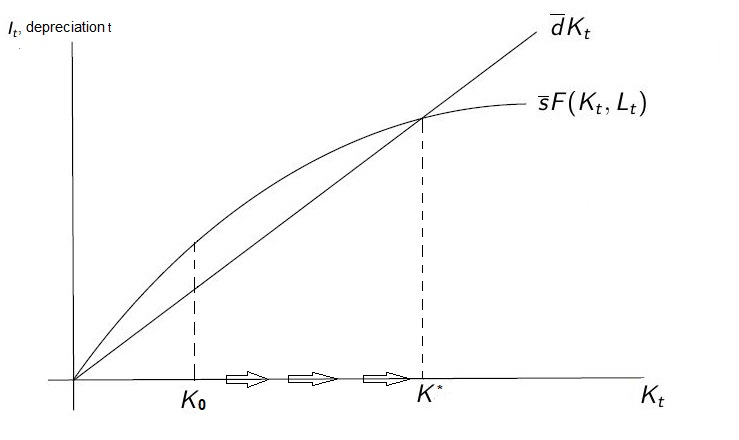
\includegraphics[scale=.6]{basic_solow_3}
\caption{$\underbrace{\Delta K_{t+1}}_{K_{t+1}>K_t}>0  \Leftrightarrow  \underbrace{\overline{s}F(K_t,L_t)}_{I_t}>\overline{d}K_t$}
\end{figure}}
\only<4>{\begin{figure}
\centering
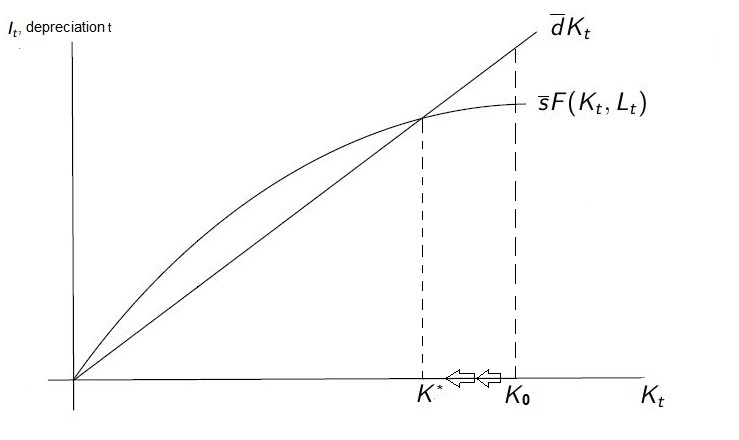
\includegraphics[scale=.6]{basic_solow_4}
\caption{$\underbrace{\Delta K_{t+1}}_{K_{t+1}<K_t}<0 \Leftrightarrow  \underbrace{\overline{s}F(K_t,L_t)}_{I_t}<\overline{d}K_t$}
\end{figure}}
\end{frame}


\begin{frame}
\frametitle{\: \: \: Dynamics of Capital Accumulation}
\toplinexlarge
\begin{itemize}
\item To simplify the analysis, we are going to assume that: $L_t=\overline{L}$  
\vspace{.11in} 
\item At $K^*$, we say that the economy is at its steady-state equilibrium.
\vspace{.11in} 
\item We can solve for $K^*$ as a function of exogenous variables and parameters:
\begin{eqnarray*}
K^*=\overline{L}\left(\frac{\overline{s}\overline{A}}{\overline{d}}\right)^{\frac{3}{2}}\\
\text{or in per capita terms: } k^*=\left(\frac{\overline{s}\overline{A}}{\overline{d}}\right)^{\frac{3}{2}}
\end{eqnarray*}
\vspace{.11in} 
\item We are also able to solve for the steady-state level of output:
\begin{eqnarray*}
 Y^*=\overline{L} \: \: \: \: \overline{A}^{\frac{3}{2}}\left(\frac{\overline{s}}{\overline{d}}\right)^{\frac{1}{2}}\\
 \text{or in per capita terms: } y^*=\overline{A}^{\frac{3}{2}}\left(\frac{\overline{s}}{\overline{d}}\right)^{\frac{1}{2}}
 \end{eqnarray*}
 \end{itemize}
 \end{frame}

\begin{frame}
\frametitle{\: \: \: Cross-country differences in $\overline{s}$ and growth}
\toplinexlarge
\begin{itemize}
\item Suppose there are two countries, CAN and ARG, with the same $\overline{A}$, $\overline{L}$, $\overline{d}$ and $K_0$ but with different $\overline{s}$
\begin{eqnarray*}
\overline{s}_{CAN}>\overline{s}_{ARG}
\end{eqnarray*}
\item At $t=0$ both countries will have the same level of output per worker:
\begin{eqnarray*}
y_0=\overline{A}\left(\frac{K_0}{\overline{L}}\right)^{\frac{1}{3}}
\end{eqnarray*}
\item However, in the long run:
\begin{eqnarray*}
y^*_{CAN}=\overline{A}^{\frac{3}{2}}\left(\frac{\overline{s}_{CAN}}{\overline{d}}\right)^{\frac{1}{2}} >\overline{A}^{\frac{3}{2}}\left(\frac{\overline{s}_{ARG}}{\overline{d}}\right)^{\frac{1}{2}}=y^*_{ARG}
\end{eqnarray*}
\end{itemize}  
\end{frame}

\begin{frame}
\frametitle{\: \: \: Cross-country differences in $\overline{s}$ and growth}
\toplinexlarge
\begin{itemize}
\item Since the starting level of GDP per capita is the same but the level of GDP per capita is higher in Canada in steady state:
\begin{itemize}
\vspace{.11in} 
\item GDP per capita on average over the long run grows faster in Canada than in Argentina.
\end{itemize}
\vspace{.11in} 
\item The main reason for this difference in growth rates is that capital accumulation is higher in Canada.
\end{itemize}  
\end{frame}

\begin{frame}
\frametitle{\: \: \: Cross-country differences in $\overline{s}$ and growth}
\toplinexlarge
\begin{figure}
\centering
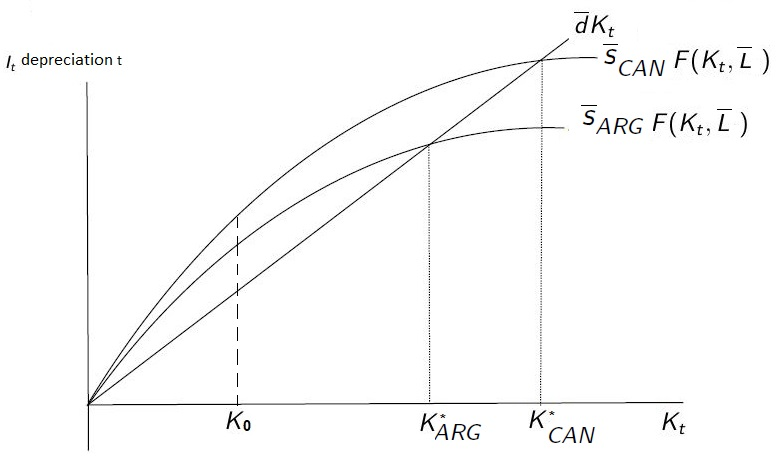
\includegraphics[scale=.68]{basic_solow_savings}
\end{figure}
\end{frame}

\begin{frame}
\frametitle{\: \: \: Solving for Equilibrium}
\toplinelarge
\begin{itemize}
\item For any $t$, the aggregate economy in the Solow Model is characterized by five equations and five unknowns ($K_t, L_t, I_t, C_t, Y_t$):
\begin{eqnarray*}
\begin{array}{ll}
\Delta K_{t+1}=\overline{s} F(K_t,L_t)-\overline{d}K_t & (\text{law of motion}) \\[1.4ex]
Y_t=\overline{A}K_t^{\frac{1}{3}}L_t^{\frac{2}{3}}& (\text{production function}) \\[1.4ex]
C_t+I_t=Y_t & (\text{resource constraint}) \\[1.4ex]
L_t=\overline{L}& (\text{labour force}) \\[1.4ex]
I_t=\overline{s} Y_t  & (\text{allocation of resources}) 
\end{array}
\end{eqnarray*}
\item For an initial level of capital, $K_0$, we can solve for the endogeneous variables in any time period.
\begin{itemize}
\vspace{.11in} 
\item Instead of solving the model for any time period, which requires a lot of algebra, we will only solve analitically for the steady state (ss) and provide graphical interpretation for other time periods.
\end{itemize}
\end{itemize}  
\end{frame}

\appendix
\section{Appendix}

\begin{frame}
\frametitle{\: \: \: Growth Algebra}\label{growth}
\toplinelarge
\begin{itemize}
\item Algebraic properties of growth rates (let the variable $i$ grow at a constant growth rate $g_i$):
\begin{eqnarray*}
\begin{array}{cl} 
z=\frac{x}{y} & \Rightarrow g_z = g_x-g_y \\
z=x \cdot y &\Rightarrow g_z = g_x+g_y \\
z=x^a \text{ (where $a$ is a constant)} & \Rightarrow g_z = a\cdot g_x
\end{array}
\end{eqnarray*}
\end{itemize}
 \hyperlink{solow}{\beamerbutton{Back}}
\end{frame}



\end{document}